\subsection{Configuration Management Plan}
This software project consists of 5 official documents including SRS, SPMP, SDD, Testing report and User Manuel), meeting agenda and minutes, and software for operating EV3 robot. All these configuration items’ standards are developed by documentation manager and monitored by quality manager. All team members are responsible for following this configuration standard during the whole project life cycle. The detail of software and testing components will be mentioned in SDD document and testing report.

\subsubsection{GitHub Repository structure and Configuration control}
The repository structure is built based on the component of the project. The highest level of repository is Code and Documentation. 
\begin{itemize}
	\item \texttt{\detokenize{...\2017-S2-SEP-PG29\Documentation}}
	\item \texttt{\detokenize{...\2017-S2-SEP-PG29\Code}}
\end{itemize}
The detail GitHub Repository structure is shown on fig.\ref{fig:GITHUB repository}.

\begin{figure}[H]
	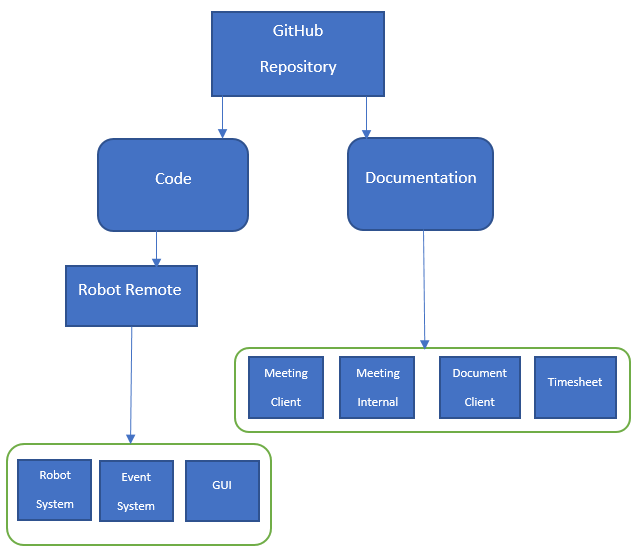
\includegraphics[width=\linewidth]{GIT.PNG}  % created using www.draw.io
	\caption{GITHUB repository}
	\label{fig:GITHUB repository}				
\end{figure}

There are three configuration directories which have special control for team members to edit. The Software components are not included in this section and will be discussed in detail on SDD document.\\
The lists of configuration control are shown as below:\\

\textbf{Library control:}\\
This library directory is for development purpose. There shall allow to store jar file only. No other file format is allowed. Team members are require to get the approval from development manager to add new jar file.\\ 
\begin{itemize}
	\item \texttt{\detokenize{...\Code\UiRemote\lib}}
\end{itemize}
\textbf{Media control:}\\
Those directory contain png file only. No other file format is allowed. Team members can feel free to add any png file for development or development purpose. Team members shall commit the change with proper message to indicate which files they are added.

\begin{itemize}
	\item \texttt{\detokenize{...Code\UiRemote\src\RobotRemote\UI\Views}}
	\item \texttt{\detokenize{...Documentation\Views}}
\end{itemize} 
\textbf{Documentation control:}\\
Those directories contain tex and pdf file only. Team members are not allowed to add any file in those directories.
Only documentation manager can add new file to those directories

\begin{itemize}
	\item \texttt{\detokenize{...Documentation\SRS}}
	\item \texttt{\detokenize{...Documentation\SPMP}}
	\item \texttt{\detokenize{...Documentation\SDD}}
\end{itemize}

\subsubsection{Configuration Naming System and version control}
Any draft of configuration items shall be followed as below naming standards:
\begin{itemize}
	\item \texttt{\detokenize{<Title>_<version>.<extension>}}\\
      		\texttt{\detokenize{For examples: SRS_v0.9.tex}}
	\item The Final version is v1.0. The draft version will be named as v0.1-v0.9.
	\item The modified date for each sub-version shall be mentioned in revision history table which is included into documents.\\
\end{itemize}

The examples of revision history for SRS-v0.9.tex is shown on Table2 :\\

\begin{table}[]
	\centering
	\caption{Revision history example}
	\label{my-labelxxxx}
	\begin{tabular}{|l|l|l|l|}
		\hline
		Name      & Date      & Version & Summary of Changes           \\ \hline
		1st Draft & 21/8/2017 & 0.9.1   & Initial Draft                \\ \hline
		2nd Draft & 22/8/2017 & 0.9.2   & Identification numbers added \\ \hline
	\end{tabular}
\end{table}


The revision table for final version shall include all the change for each version. After final version released, any change is required a change request which is mentioned in section 8.3.\\


The meeting agenda and meeting minutes shall follow as below naming system:\\
\texttt{\detokenize{<Title>_<Type>_<week>.<extension>}}\\
\begin{itemize}
\item Title: Agenda or Minutes
\item Type: Client or Internal
\end{itemize}
\texttt{\detokenize{For example: agenda_client_week3.tex, minutes_internal_week3.tex}} \\\\
Usually, there are only one client meeting and internal group meeting per week. If there are any emergency meeting, the date should be included.\\\\
\texttt{\detokenize{For example: agenda_internal_week3_17082017.tex}}\\
\texttt{\detokenize{The date format shall be <days><months><year>}}\\

\subsubsection{Change request handling}
There are two types change request handling. Documentation and Software change request handling.\\\\
\textbf{Documentation:}\\
The Documents will be divided by documentation manager into difference sub-tasks for each team member to edit their own parts. 
\begin{itemize}
\item Team members can make any change on their own part before the final version release. 

\item Team members is required to edit the revision table to record their change on the document. 

\item The documentation review meeting will be held by documentation manager to review all the changes on the document before releasing final version.

\item The change on Final version's document is not allowed without discussion in another new review meeting. 
\end{itemize}
\textbf{Software:}
\begin{itemize}
\item Team member must need to create new branch in github repository to make a change or add new function on software. 
\item The change on this branch must not affect master branch.
\item Regular software review meeting will be held by development manager to review all the team member’s work and discuss the potential issue before merging the work to master branch.
\end{itemize}

\newpage

% 8.2
% Documentation plan
% List the documents to be prepared. Give details on the document template to be used (whereappropriate). Describe the preparation and review process for documents.

\subsection{Documentation Plan}
The documentation plan involves several key documents and revision processes that ensure the quality of the overall project is kept at a high level.

\subsubsection{SRS}
The Software Requirements Specification will be constructed using the \textit{IEEE Recommended Practice for Software Requirements Specifications} standard provided by the IEEE.\\

\textbf{Structure}
\begin{enumerate}
	\item[-] Revision History
	\item Introduction
	\item Overall Description
	\item User Requirements
	\item System Features
	\item External Interface Requirements
	\item Other Non-Functional Requirements
	\item Other Requirements
	\item[-] Appendix A: Glossary
	\item[-] Appendix B: Analysis Models
	\item[-] Appendix C: Issues List
\end{enumerate}

\subsubsection{SPMP}
The Software Project Management Plan shall be constructed with the following structure:\\

\textbf{Structure}
\begin{enumerate}
	\item[-] Revision History
	\item Introduction
	\item References
	\item Definition
	\item Project Organisation
	\item Risk Management
	\item Process Model
	\item Work Plan
	\item Supporting Plans
	\item Appendices
\end{enumerate}
	
\subsubsection{SDD}
The the Software Design Document is as follows:\\

\textbf{Structure}
\begin{enumerate}
	\item[-] Revision History
	\item Introduction
	\item System Overview
	\item System Architecture and Components Design
	\item Data Design
	\item Design Details
	\item Human Interface Design
	\item Resource Estimates
	\item Definitions, Acronyms, and Abbreviations
	\item Appendices
\end{enumerate}

\subsubsection{Client Meetings}
The formal documentation for client meetings is crucial as it is a record of what ideas and decisions were made that will affect the entire project. \\

\textbf{Agenda}\\
An important document for client meetings is the client meeting agenda. This document provides both parties with a common understanding of what purpose of the meeting is and the items that will be discussed. Structure of the agenda is as follows:

\begin{itemize}
	\item Attendance
	\item Progress summary of the project
	\item Points from last meeting
	\item New questions for this meeting
	\item Questions for the project team
\end{itemize}

\textbf{Minutes}\\
Prior to each client meeting, a group member will be designated to record the minutes of the meeting. They're task is to record as much important information in the meeting as they can including but not limited to the following:

\begin{itemize}
	\item Attendance
	\item Questions we asked the client, and answers
	\item Questions the client asked us
	\item Problems needed to be addressed for next meeting
	\item Ideas, or possible solutions during discussion
\end{itemize}

\subsubsection{Internal Meetings}
Although internal meetings are less formal, we plan to produce an meeting agenda and record meeting minutes. Similar to the client meeting agenda, the internal meeting agenda format should allow for everyone to prepare for the meeting and provide a much more efficient discussion. Additionally, the internal versions will contain enough information that people can refer to at a later date.

\subsubsection{Timesheets}
Another internal document is the group member timesheet. This is a document which is used for internal tracking of group member participation and progress. It should be a record of the time spent on what tasks, and should be filled out on a weekly biases and saved in the Github repository.

\subsubsection{Document Review Processes}
Several revision processes will be used in order to enhance the quality of the documents planned out. These processes include:

\begin{itemize}
\item Brainstorming
\item Spelling and Grammar Review
\item Collaborative and traceable document editing through Github with latex
\item Team member review
\end{itemize}

% 8.3
% Quality assurance plan 
% This should include a description of your verification and validation (V&V) process. You should also list any standards (this may include in coding standards for example) that you intend to use the process that you will put in place to ensure you have correctly followed the standard. You might also want to include details on the software review and inspection processes that you intend to adopt.


\subsection{Quality Assurance Plan}
The quality assurance of the project is managed using a combination of several methods. The following subsections detail the plans used throughout the project.

\subsubsection{Coding Standards}
Throughout the project a common set of coding conventions are to be used. This includes the following points:\\

\textbf{Code Formatting}\\
All code that is committed to the repository is to be formatted with respect to the \textit{Google Java Style Guide} This is automated through the IDE chosen, which is Jetbrains IntelliJ 2017.\\

\subsubsection{Software Review Process}
\textbf{Unit Testing}\\
With an effort to provide quality code that has proven functionality, a testing plan will be carried out, in which all functional code will have associated unit tests.\\

\textbf{Code Review}\\
Finally, all code that is committed to the repository is to be reviewed before it is merged to the master branch.

\subsubsection{Traceability}
\textbf{Github}\\
To ensure traceability throughout the duration of the project, the Github repository will be the primary source of information. This will provide a detailed history of changes to each document and which team members made them. \\

\textbf{Slack}\\
Additionally, Slack will be used for internal correspondence between the project team. This also allows for traceability of conversations between the team, which helps document ideas and features for the project.

\subsubsection{Roles}
As described in section \ref{roles}, each group member is responsible for a different area of the project. This dependency on specialised roles, is offset by the processes used to improve the quality of the project, as all group members will get the chance to work with the code, testing, documentation and project management. This additionally helps with redundancy, and improves the resilience of the project, with respect to unforeseen changes.

\begin{enumerate}
	\item[Pavi] - Project Manager
	\item[Ben] - Documentation Manager
	\item[Issac] - Testing Manager
	\item[Sammy] - IT Manager
	\item[John] - Development Manager
	\item[Sean] - Quality Manager
\end{enumerate}
